\documentclass[12pt]{beamer}
\usepackage{tikz}

\usetikzlibrary{%
  calc,%
  arrows,%
  decorations,%
  decorations.markings%
}
\usecolortheme{crane}
\usefonttheme{serif}

\title{Distributed bitonic sort}
\author{Roberto Bonvallet \\ \texttt{roberto.bonvallet@usm.cl}}
\institute{CTI-HPC}
\date{\today}

\tikzstyle{process}=[draw, circle, inner sep=1ex]
\tikzstyle{front}=[xshift=-0.2cm, yshift=-0.1cm]
\tikzstyle{back} =[xshift= 0.2cm, yshift= 0.1cm, opacity=0.5]
\tikzstyle{comm}=[ultra thick, red!90!black, <->]
\tikzstyle{lsort}=[circle, font=\footnotesize,
%  fill opacity=.8,
  fill=orange!90!black]
\tikzstyle{bitonic}=[
  rounded corners=0.7cm, ultra thick,
  blue!90!black, fill=blue!50!white, fill opacity=0.2
]
\tikzstyle{sorted}=[
  rounded corners=0.7cm, ultra thick,
  orange!90!black, fill=orange!50!white, fill opacity=0.2
]

\tikzstyle{ordered}=[
  decoration={markings, mark=at position 0.6 with {\arrow[line width=5pt]{angle 90 reversed}}},
  postaction={decorate}
]

% for debugging
\tikzstyle{frontgrid}=[orange!50!blue, front, opacity=0.4]
\tikzstyle{backgrid}= [orange!50!blue, back , opacity=0.3]

% for "production"
\tikzstyle{frontgrid}=[front, opacity=0.05]
\tikzstyle{backgrid}= [back,  opacity=0.05]

\newcommand\fori{\foreach\i in {0,1}}
\newcommand\forij{\foreach\i in {0,1} \foreach\j in {0,1}}
\newcommand\fork{\foreach \k/\where in {0/front, 1/back}}
\newcommand\asc{\ensuremath{\nearrow}}
\newcommand\desc{\ensuremath{\searrow}}

\begin{document}

  \begin{frame}
    \titlepage
  \end{frame}

  \begin{frame}
    \begin{center}
      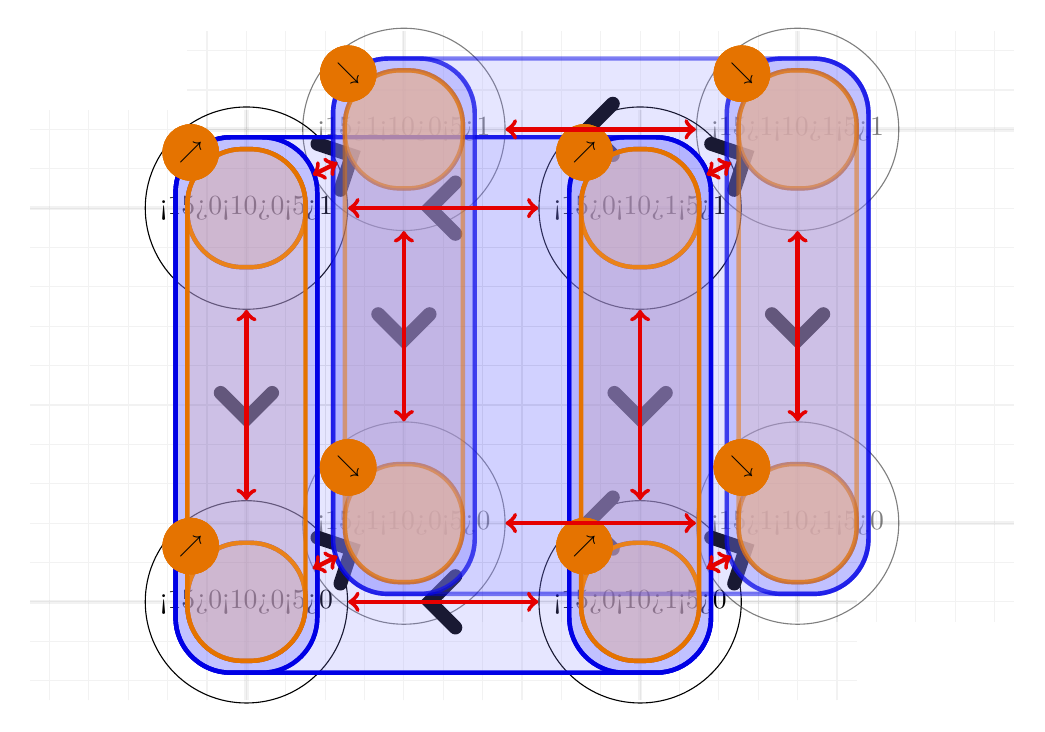
\begin{tikzpicture}[scale=5]

        % reference grid
        \begin{scope}
          \def\xf{.55}
          \def\yf{.25}
          \draw[frontgrid, ultra thick] (-\xf, -\yf) grid (1 + \xf, 1 + \yf);
          \draw[frontgrid, step=0.1cm ] (-\xf, -\yf) grid (1 + \xf, 1 + \yf);
          \draw[backgrid,  ultra thick] (-\xf, -\yf) grid (1 + \xf, 1 + \yf);
          \draw[backgrid,  step=0.1cm ] (-\xf, -\yf) grid (1 + \xf, 1 + \yf);
        \end{scope}

        % map names to slides
        \def\sortA        {2}
        \def\afterSortA   {3}
        \def\beforeSplitA {4}
        \def\commA        {5}
        \def\afterSplitA  {6}
        \def\sortB        {7}
        \def\afterSortB   {8}
        \def\beforeSplitB {9}
        \def\commB        {10}
        \def\afterSplitB  {11}
        \def\sortC        {12}
        \def\afterSortC   {13}
        \def\beforeSplitC {14}
        \def\commC        {15}
        \def\afterSplitC  {16}

        % process nodes
        \fork {
          \begin{scope}[\where]
            \forij
              \node[process] (p\k\i\j) at (\i, \j) {
                \alert<\commC>{\k}%
                \alert<\commB>{\i}%
                \alert<\commA>{\j}%
              };
          \end{scope}
        }

        % node connections
        \forij \draw (p\i\j0) -- (p\i\j1);
        \forij \draw (p\i0\j) -- (p\i1\j);
        \forij \draw (p0\i\j) -- (p1\i\j);

        % connections decorated with mutual ordering between nodes
        \forij \draw<\afterSplitA, \sortB, \beforeSplitB>[ordered] (p\i\j0) -- (p\i\j1);
        \forij \draw<\afterSplitB, \sortC, \beforeSplitC>[ordered] (p\i0\j) -- (p\i1\j);
        \forij \draw<\afterSplitC>                       [ordered] (p0\i\j) -- (p1\i\j);

        \def\dr{.15}
        \def\dR{.18}

        % bitonicity among vertical neighbors
        \fork {
          \draw<\beforeSplitA, \commA>[\where, bitonic] (0 - \dR, 1 + \dR) rectangle (0 + \dR, 0 - \dR);
          \draw<\beforeSplitA, \commA>[\where, bitonic] (1 - \dR, 1 + \dR) rectangle (1 + \dR, 0 - \dR);
        }

        % bitonicity after first split
        \fork\forij
          \draw<\afterSplitA>[bitonic, \where] (\i - \dr, \j - \dr) rectangle (\i + \dr, \j + \dr);

        % bitonicity among front and back neighbors
        \fork \draw<\beforeSplitB, \commB>[\where,  bitonic] (0 - \dR, 0 - \dR) rectangle (1 + \dR, 1 + \dR);

        % bitonicity after second split
        \fork {
          \draw<\afterSplitB>[\where, bitonic] (0 - \dR, 1 + \dR) rectangle (0 + \dR, 0 - \dR);
          \draw<\afterSplitB>[\where, bitonic] (1 - \dR, 1 + \dR) rectangle (1 + \dR, 0 - \dR);
        }

        % ordering after first local sort
        \fork\forij
          \draw<\afterSortA, \beforeSplitA>[sorted, \where] (\i - \dr, \j - \dr) rectangle (\i + \dr, \j + \dr);
        \forij \node<\afterSortA, \beforeSplitA> [above left of=p\i\j0] {\asc};
        \forij \node<\afterSortA, \beforeSplitA> [above left of=p\i\j1] {\desc};

        % ordering after second local sort
        \fork {
          \draw<\afterSortB, \beforeSplitB>[\where, sorted] (0 - \dr, 1 + \dr) rectangle (0 + \dr, 0 - \dr);
          \draw<\afterSortB, \beforeSplitB>[\where, sorted] (1 - \dr, 1 + \dr) rectangle (1 + \dr, 0 - \dr);
        }
        \fori \node<\afterSortB, \beforeSplitB> [above left of=p\i01] {\asc};
        \fori \node<\afterSortB, \beforeSplitB> [above left of=p\i11] {\desc};

        % first local sorting stage
        \forij \node<\sortA> [lsort, above left of=p\i\j0] {\asc};
        \forij \node<\sortA> [lsort, above left of=p\i\j1] {\desc};

        % second local sorting stage
        \forij \node<\sortB> [lsort, above left of=p\i0\j] {\asc};
        \forij \node<\sortB> [lsort, above left of=p\i1\j] {\desc};

        % third local sorting stage
        \forij \node<\sortC> [lsort, above left of=p0\i\j] {\asc};
        \forij \node<\sortC> [lsort, above left of=p1\i\j] {\desc};

        % communication between nodes
        \forij \draw<\commA>[comm] (p\i\j0) -- (p\i\j1);
        \forij \draw<\commB>[comm] (p\i0\j) -- (p\i1\j);
        \forij \draw<\commC>[comm] (p0\i\j) -- (p1\i\j);

      \end{tikzpicture}
    \end{center}
  \end{frame}

  \begin{frame}
    \frametitle{}
  \end{frame}

\end{document}

